% questions.tex —— 2007 年·普通高等学校招生考试·浙江卷·文科 · 题目内容片段（无答案）
% 由 tools/generate_projects.py 依来源总账自 2007/2007_数学真题_浙江文_试题.md 生成，勿手改（改源 MD 后重跑）


状态：needs-review；依固定候选 PDF 两页（印刷页 419–420）三栏图像以 300 dpi 渲染逐题核验，图形已矢量重绘，正式构建与逐页验收待完成。源未列各题分值，不补分值。

\gkpart{一、选择题}

\begin{question}
\gkti{1}设全集 $U=\{1,3,5,6,8\}$，$A=\{1,6\}$，$B=\{5,6,8\}$，则 $(\complement_UA)\cap B=$（　）

（A）$\{6\}$

（B）$\{5,8\}$

（C）$\{6,8\}$

（D）$\{3,5,6,8\}$

\end{question}
\begin{question}
\gkti{2}已知 $\cos\left(\dfrac{\pi}{2}+\varphi\right)=\dfrac{\sqrt3}{2}$，且 $|\varphi|<\dfrac{\pi}{2}$，则 $\tan\varphi=$（　）

（A）$-\dfrac{\sqrt3}{3}$

（B）$\dfrac{\sqrt3}{3}$

（C）$-\sqrt3$

（D）$\sqrt3$

\end{question}
\begin{question}
\gkti{3}“$x>1$”是“$x^2>x$”的（　）

（A）充分而不必要条件

（B）必要而不充分条件

（C）充分必要条件

（D）既不充分也不必要条件

\end{question}
\begin{question}
\gkti{4}直线 $x-2y+1=0$ 关于直线 $x=1$ 对称的直线方程是（　）

（A）$x+2y-1=0$

（B）$2x+y-1=0$

（C）$2x+y-3=0$

（D）$x+2y-3=0$

\Needspace{0.4\textheight}
\end{question}
\begin{question}
\gkti{5}要在边长为 $16$ 米的正方形草坪上安装喷水龙头，使整个草坪都能喷洒到水。假设每个喷水龙头的喷洒范围都是半径为 $6$ 米的圆面，则需安装这种喷水龙头的个数最少是（　）
\nopagebreak[4]
\begin{center}% 2007 年浙江卷文科第 5 题：边长 16 米的正方形草坪与喷水龙头示意。
% 来源 PDF：gaokaomath-src/普通高考/2007/2007浙江文.pdf
% SHA-256：31c1d0d79ba11a3644a27b5ee3781f52caaf831209e8da63ddd8d7019cd06995
% 原页：2007浙江文.pdf 第 1 页（A3 三栏）第 1 栏，书页码 419。
% 重绘依据：按原页正方形草坪与中心喷水圆面的透视重绘。
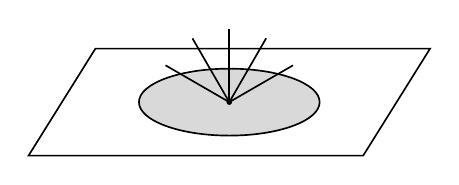
\begin{tikzpicture}[scale=0.85, semithick,
  every node/.style={inner sep=1pt}]

  % 正方形草坪（斜投影）
  \draw (0,0) -- (5,0) -- (6,1.6) -- (1,1.6) -- cycle;

  % 喷水圆面
  \fill[gray!30] (3,0.8) ellipse (1.35 and 0.5);
  \draw (3,0.8) ellipse (1.35 and 0.5);
  \fill (3,0.8) circle (1.2pt);

  % 水花射线
  \foreach \a in {30,60,90,120,150} {
    \draw (3,0.8) -- ++(\a:1.1);
  }
\end{tikzpicture}
\end{center}
\nopagebreak[4]
（A）$6$

（B）$5$

（C）$4$

（D）$3$

\end{question}
\begin{question}
\gkti{6}$\left(\sqrt x-\dfrac1x\right)^9$ 展开式中的常数项是（　）

（A）$-36$

（B）$36$

（C）$-84$

（D）$84$

\end{question}
\begin{question}
\gkti{7}若 $P$ 是两条异面直线 $l$，$m$ 外的任意一点，则（　）

（A）过点 $P$ 有且仅有一条直线与 $l$，$m$ 都平行

（B）过点 $P$ 有且仅有一条直线与 $l$，$m$ 都垂直

（C）过点 $P$ 有且仅有一条直线与 $l$，$m$ 都相交

（D）过点 $P$ 有且仅有一条直线与 $l$，$m$ 都异面

\end{question}
\begin{question}
\gkti{8}甲，乙两人进行乒乓球比赛，比赛规则为“$3$ 局 $2$ 胜”，即以先赢 $2$ 局者为胜。根据经验，每局比赛中甲获胜的概率为 $0.6$，则本次比赛甲获胜的概率是（　）

（A）$0.216$

（B）$0.36$

（C）$0.432$

（D）$0.648$

\end{question}
\begin{question}
\gkti{9}若非零向量 $\boldsymbol a$，$\boldsymbol b$ 满足 $|\boldsymbol a-\boldsymbol b|=|\boldsymbol b|$，则（　）

（A）$|2\boldsymbol b|<|\boldsymbol a-2\boldsymbol b|$

（B）$|2\boldsymbol b|<|\boldsymbol a-2\boldsymbol b|$

（C）$|2\boldsymbol a|>|2\boldsymbol a-\boldsymbol b|$

（D）$|2\boldsymbol a|<|2\boldsymbol a-\boldsymbol b|$

\end{question}
\begin{question}
\gkti{10}已知双曲线 $\dfrac{x^2}{a^2}-\dfrac{y^2}{b^2}=1$（$a>0$，$b>0$）的左、右焦点分别为 $F_1$，$F_2$，$P$ 是准线上一点，且 $PF_1\perp PF_2$，$|PF_1|\cdot|PF_2|=4ab$，则双曲线的离心率是（　）

（A）$\sqrt2$

（B）$\sqrt3$

（C）$2$

（D）$3$

\end{question}
\gkpart{二、填空题}

\begin{question}
\gkti{11}函数 $y=\dfrac{x^2}{x^2+1}$（$x\in\mathbf R$）的值域是\gkblank{}。

\end{question}
\begin{question}
\gkti{12}若 $\sin\theta+\cos\theta=\dfrac15$，则 $\sin2\theta$ 的值是\gkblank{}。

\end{question}
\begin{question}
\gkti{13}某校有学生 $2000$ 人，其中高三学生 $500$ 人。为了解学生的身体素质情况，采用按年级分层抽样的方法，从该校学生中抽取一个 $200$ 人的样本。则样本中高三学生的人数为\gkblank{}。

\end{question}
\begin{question}
\gkti{14}$z=2x+y$ 中的 $x$，$y$ 满足约束条件 $\begin{cases}x-2y+5\geqslant0,\\ 3-x\geqslant0,\\ x+y\geqslant0,\end{cases}$ 则 $z$ 的最小值是\gkblank{}。

\end{question}
\begin{question}
\gkti{15}曲线 $y=x^3-2x^2-4x+2$ 在点 $(1,-3)$ 处的切线方程是\gkblank{}。

\end{question}
\begin{question}
\gkti{16}某书店有 $11$ 种杂志，$2$ 元 $1$ 本的 $8$ 种，$1$ 元 $1$ 本的 $3$ 种。小张用 $10$ 元钱买杂志（每种至多买一本，$10$ 元钱刚好用完），则不同买法的种数是\gkblank{}。（用数字作答）

\end{question}
\begin{question}
\gkti{17}已知点 $O$ 在二面角 $\alpha-AB-\beta$ 的棱上，点 $P$ 在 $\alpha$ 内，且 $\angle POB=45^\circ$。若对于 $\beta$ 内异于 $O$ 的任意一点 $Q$，都有 $\angle POQ\geqslant45^\circ$，则二面角 $\alpha-AB-\beta$ 的大小是\gkblank{}。

\end{question}
\gkpart{三、解答题}

\begin{question}
\gkti{18}已知 $\triangle ABC$ 的周长为 $\sqrt2+1$，且 $\sin A+\sin B=\sqrt2\sin C$。

（1）求边 $AB$ 的长；

（2）若 $\triangle ABC$ 的面积为 $\dfrac16\sin C$，求角 $C$ 的度数。

\end{question}
\begin{question}
\gkti{19}已知数列 $\{a_n\}$ 中的相邻两项 $a_{2k-1}$，$a_{2k}$ 是关于 $x$ 的方程 $x^2-(3k+2^k)x+3k\cdot2^k=0$ 的两个根，且 $a_{2k-1}\leqslant a_{2k}$（$k=1,2,3,\cdots$）。

（1）求 $a_1$，$a_3$，$a_5$，$a_7$ 及 $a_{2n}$（$n\geqslant4$）（不必证明）；

（2）求数列 $\{a_n\}$ 的前 $2n$ 项和 $S_{2n}$。

\Needspace{0.4\textheight}
\end{question}
\begin{question}
\gkti{20}在如图所示的几何体中，$EA\perp$ 平面 $ABC$，$DB\perp$ 平面 $ABC$，$AC\perp BC$，且 $AC=BC=BD=2AE$，$M$ 是 $AB$ 的中点。

（1）求证：$CM\perp EM$；

（2）求 $DE$ 与平面 $EMC$ 所成角的正切值。
\nopagebreak[4]
\begin{center}% 2007 年浙江卷文科第 20 题：EA、DB 均垂直于平面 ABC，AC⊥BC，M 为 AB 中点。
%   按 AC=BC=2、AE=1、BD=2 的示意比例绘制。
% 来源 PDF：gaokaomath-src/普通高考/2007/2007浙江文.pdf
% SHA-256：31c1d0d79ba11a3644a27b5ee3781f52caaf831209e8da63ddd8d7019cd06995
% 原页：2007浙江文.pdf 第 2 页（A3 三栏）第 1 栏，书页码 420。
% 重绘依据：按原页 C、A、B 底面与 E、D 的竖直位置重绘。
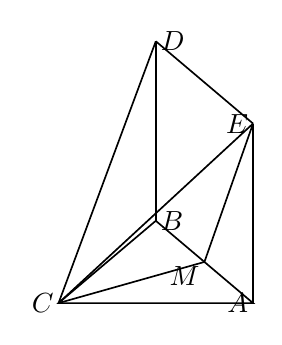
\begin{tikzpicture}[scale=0.95, semithick,
  every node/.style={inner sep=1.5pt}]

  \coordinate (C) at (0,0);
  \coordinate (A) at (2.6,0);
  \coordinate (B) at (1.3,1.1);
  \coordinate (E) at (2.6,2.4);
  \coordinate (D) at (1.3,3.5);
  \coordinate (M) at (1.95,0.55);

  % 底面
  \draw (C) -- (A) -- (B) -- cycle;
  % 竖直线
  \draw (A) -- (E);
  \draw (B) -- (D);
  % 上方连线
  \draw (E) -- (D);
  \draw (E) -- (C);
  \draw (D) -- (C);
  % 中点 M 相关
  \draw (C) -- (M);
  \draw (E) -- (M);

  \node[left] at (C) {$C$};
  \node[left] at (A) {$A$};
  \node[right] at (B) {$B$};
  \node[left] at (E) {$E$};
  \node[right] at (D) {$D$};
  \node[below left] at (M) {$M$};
\end{tikzpicture}
\end{center}
\nopagebreak[4]
\Needspace{0.4\textheight}
\end{question}
\begin{question}
\gkti{21}如图，直线 $y=kx+b$ 与椭圆 $\dfrac{x^2}{4}+y^2=1$ 交于 $A$，$B$ 两点，记 $\triangle AOB$ 的面积为 $S$。

（1）求在 $k=0$，$0<b<1$ 的条件下，$S$ 的最大值；

（2）当 $|AB|=2$，$S=1$ 时，求直线 $AB$ 的方程。
\nopagebreak[4]
\begin{center}% 2007 年浙江卷文科第 21 题：直线 y=kx+b 与椭圆 x^2/4+y^2=1 交于 A、B，
%   记三角形 AOB 的面积为 S。
% 来源 PDF：gaokaomath-src/普通高考/2007/2007浙江文.pdf
% SHA-256：31c1d0d79ba11a3644a27b5ee3781f52caaf831209e8da63ddd8d7019cd06995
% 原页：2007浙江文.pdf 第 2 页（A3 三栏）第 2 栏，书页码 420。
% 重绘依据：按原页椭圆、割线与 A、B、O 的位置重绘。
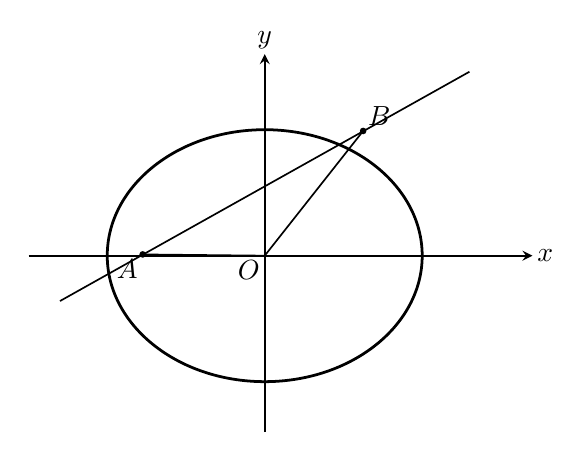
\begin{tikzpicture}[x=1.0cm, y=1.6cm, semithick,
  every node/.style={inner sep=1.5pt}]

  \draw[->,>=stealth] (-3.0,0) -- (3.4,0) node[right] {$x$};
  \draw[->,>=stealth] (0,-1.4) -- (0,1.6) node[above] {$y$};
  \node[below left] at (0,0) {$O$};

  % 椭圆 x^2/4+y^2=1
  \draw[line width=1pt] (0,0) ellipse (2 and 1);

  % 割线 y = 0.35x + 0.55（示意）
  \draw (-2.6,-0.36) -- (2.6,1.46);
  \coordinate (A) at (-1.55,0.01);
  \coordinate (B) at (1.25,0.99);
  \fill (A) circle (1.2pt);
  \fill (B) circle (1.2pt);
  \node[below left] at (A) {$A$};
  \node[above right] at (B) {$B$};

  \draw (A) -- (0,0) -- (B);
\end{tikzpicture}
\end{center}
\nopagebreak[4]

\end{question}